\documentclass[10pt]{beamer}
\usepackage{graphicx}
\usepackage{enumitem}
\usepackage{tikz}
\usetikzlibrary{arrows.meta,positioning,decorations.pathreplacing}
\usepackage{pifont}
% Prefetcher colours, same as in the charts (colour-blind safe)
\definecolor{cIP}{HTML}{2A78D6}
\definecolor{cBOP}{HTML}{EB811B}
\definecolor{cBerti}{HTML}{1BAF7A}
\newcommand{\msg}[1]{%
  \begin{tikzpicture}
    \node[fill=mDarkTeal!8, draw=mDarkTeal!40, rounded corners=3pt,
          inner xsep=8pt, inner ysep=6pt, text width=0.92\linewidth, align=center]
      {\normalsize #1};
  \end{tikzpicture}}
% Reveal TikZ parts step by step: [visible on=<2->]
\tikzset{invisible/.style={opacity=0, text opacity=0},
  visible on/.style={alt={#1{}{invisible}}},
  alt/.code args={<#1>#2#3}{\alt<#1>{\pgfkeysalso{#2}}{\pgfkeysalso{#3}}}}
\newcommand{\good}{{\color{mLightGreen}\ding{51}}}
\newcommand{\bad}{{\color{mLightBrown}\ding{55}}}

\usetheme{metropolis}

% Fira Sans with any engine: XeLaTeX/LuaLaTeX get it from Metropolis,
% pdflatex needs the FiraSans package. Match Metropolis: Light text,
% Regular for bold, lining (not old-style) digits.
\usepackage{iftex}
\ifPDFTeX
  \usepackage[T1]{fontenc}
  \usepackage[sfdefault,light,lining]{FiraSans}
  \makeatletter\def\bfseries@sf{m}\makeatother
\fi

% Title page: name stands out, details recede
\setbeamerfont{author}{size=\large}
\setbeamerfont{institute}{size=\normalsize}
\setbeamerfont{frametitle}{size=\Large}
% \setbeamercolor{institute}{fg=black}
% \setbeamertemplate{institute}{\vspace*{0mm}\insertinstitute\par}
\setbeamersize{text margin left=1.5cm, text margin right=1.5cm}
\setlist[itemize,1]{label=\small$\bullet$}
% slide numbers bottom-right (Metropolis default footer)
\setbeamertemplate{frame numbering}[counter]
\setbeamertemplate{navigation symbols}{}

\title{LoGO: Combining Local Deltas and Global Offsets for Data Prefetching}
\subtitle{CS683 Project\\Checkpoint 1}
\author{Mradul Sonkar\\[0.05cm]{\normalsize\color{black!65}23B0980}}
\institute{Instructor: Biswabandan Panda\\{\small \normalsize\color{black!65}{Department of Computer Science and Engineering, IIT Bombay}}}
\date{}

\begin{document}
\maketitle

% ---------------------------------------------------------------------------
\begin{frame}{Why Data Prefetching?}
  \centering
  {\large Memory is far from the CPU}\\[0.4cm]

  % Latency ladder: each level is slower; numbers from our simulated machine
  \begin{tikzpicture}[
      lvl/.style={draw=none, rounded corners=2pt, minimum height=0.9cm,
                  font=\normalsize, text=white, align=center},
      lat/.style={font=\small, text=black!70},
      >={Stealth[length=2mm]}]
    \node[lvl, fill=mDarkTeal!45, minimum width=1.2cm] (cpu) {CPU};
    \node[lvl, fill=mDarkTeal!60, minimum width=1.2cm, right=0.35cm of cpu] (l1) {L1};
    \node[lvl, fill=mDarkTeal!75, minimum width=1.3cm, right=0.35cm of l1] (l2) {L2};
    \node[lvl, fill=mDarkTeal!90, minimum width=1.4cm, right=0.35cm of l2] (llc) {LLC};
    \node[lvl, fill=mLightBrown, minimum width=2.4cm, right=0.35cm of llc] (dram) {DRAM};
    \foreach \a/\b in {cpu/l1, l1/l2, l2/llc, llc/dram}
      \draw[->, black!50, thick] (\a) -- (\b);
    \node[lat, below=0.15cm of l1]   {5 cyc};
    \node[lat, below=0.15cm of l2]   {15 cyc};
    \node[lat, below=0.15cm of llc]  {35 cyc};
    \node[lat, below=0.15cm of dram] {\textbf{300+ cyc}};
  \end{tikzpicture}\\[0.6cm]

  % The idea in one line
  \begin{tikzpicture}
    \node[fill=mDarkTeal!8, draw=mDarkTeal!40, rounded corners=3pt,
          inner xsep=10pt, inner ysep=8pt, text width=0.8\linewidth, align=center]
      {\large \textbf{Prefetcher:} guess the next address, fetch it early};
  \end{tikzpicture}\\[0.6cm]

  % Why it matters, from our runs
  \begin{columns}[T]
    \begin{column}{0.45\textwidth}
      \centering
      {\LARGE\color{mLightGreen}\textbf{1.74$\times$}}\\[0.1cm]
      {\small faster with Berti\\(Trace - \textbf{fotonik3d})}
    \end{column}
    \begin{column}{0.45\textwidth}
      \centering
      {\LARGE\color{mLightBrown}\textbf{0.065}}\\[0.1cm]
      {\small instructions/cycle without one\\(Trace - \textbf{pr}, waiting on memory)}
    \end{column}
  \end{columns}
\end{frame}

% ---------------------------------------------------------------------------
\begin{frame}{Two Ways to Guess}
  \tikzset{
    ip/.style={draw=none, fill=mDarkTeal!80, text=white, rounded corners=2pt,
               minimum width=1.1cm, minimum height=0.6cm, font=\small},
    off/.style={draw=none, fill=mLightGreen!85!black, text=white, rounded corners=2pt,
                minimum width=0.9cm, minimum height=0.6cm, font=\small},
    gone/.style={draw=black!35, dashed, text=black!45, rounded corners=2pt,
                 minimum width=0.9cm, minimum height=0.6cm, font=\small},
    >={Stealth[length=2mm]}}

  \begin{columns}[T]
    % ---- Local ------------------------------------------------------------
    \begin{column}{0.48\textwidth}
      \centering
      {\large\textbf{Local}}\\
      {\small one delta \emph{per instruction} (Berti)}\\[0.35cm]
      \begin{tikzpicture}
        \node[ip] (a) at (0, 0)    {IP A};
        \node[ip] (b) at (0,-0.85) {IP B};
        \node[ip] (c) at (0,-1.7)  {IP C};
        \node[off]  (da) at (2.2, 0)    {+2};
        \node[off]  (db) at (2.2,-0.85) {+5};
        \node[gone] (dc) at (2.2,-1.7)  {?};
        \draw[->, thick, black!55] (a) -- (da);
        \draw[->, thick, black!55] (b) -- (db);
        \draw[->, thick, black!25, dashed] (c) -- (dc);
      \end{tikzpicture}\\[0.35cm]
      \begin{tabular}{@{}l@{\hspace{0.15cm}}l@{}}
        \bad  & silent when unsure \\
        \good & 93\% accurate
      \end{tabular}
    \end{column}
    % ---- Global -----------------------------------------------------------
    \begin{column}{0.48\textwidth}
      \centering
      {\large\textbf{Global}}\\
      {\small one offset \emph{for everything} (BOP)}\\[0.35cm]
      \begin{tikzpicture}
        \node[ip] (a) at (0, 0)    {IP A};
        \node[ip] (b) at (0,-0.85) {IP B};
        \node[ip] (c) at (0,-1.7)  {IP C};
        \node[off, fill=mLightBrown, minimum height=2.3cm] (d) at (2.2,-0.85) {+D};
        \foreach \x in {a,b,c} \draw[->, thick, black!55] (\x) -- (d);
      \end{tikzpicture}\\[0.35cm]
      \begin{tabular}{@{}l@{\hspace{0.15cm}}l@{}}
        \good & always guesses \\
        \bad  & 48\% accurate
      \end{tabular}
    \end{column}
  \end{columns}

  \vfill
  {\scriptsize\color{black!75}
   $\ast$ Accuracy = of all lines prefetched, the share the program actually used.\\
   $\ast$ Average over 9 program traces: 6 standard CPU benchmarks (e.g.\ mcf, lbm)
   and 3 graph algorithms.\par}
\end{frame}

\begin{frame}{Problem Statement}
  \centering
  % Picture: Berti handles IP A, is silent on IP C; can the global offset step in?
  \begin{tikzpicture}[
      ip/.style={draw=none, fill=mDarkTeal!80, text=white, rounded corners=2pt,
                 minimum width=1.1cm, minimum height=0.6cm, font=\small},
      off/.style={draw=none, fill=mLightGreen!85!black, text=white, rounded corners=2pt,
                  minimum width=0.9cm, minimum height=0.6cm, font=\small},
      gone/.style={draw=black!35, dashed, text=black!45, rounded corners=2pt,
                   minimum width=0.9cm, minimum height=0.6cm, font=\small},
      lbl/.style={font=\small, text=black!60},
      >={Stealth[length=2mm]}]
    \node[ip]   (a)  at (0, 0)    {IP A};
    \node[off]  (da) at (2.4, 0)  {+2};
    \node[lbl, right=0.25cm of da] {Berti: confident};
    \node[ip]   (c)  at (0,-1.0)  {IP C};
    \node[gone] (dc) at (2.4,-1.0) {?};
    \node[lbl, right=0.25cm of dc] {Berti: silent \(\rightarrow\) miss};
    \node[off, fill=mLightBrown] (d) at (2.4,-2.1) {+D};
    \node[lbl, right=0.25cm of d] {global offset: use it here?};
    \draw[->, thick, black!55] (a) -- (da);
    \draw[->, thick, black!25, dashed] (c) -- (dc);
    \draw[->, thick, mLightBrown, dashed] (c.south east) to[bend right=15] (d.west);
  \end{tikzpicture}\\[0.3cm]

  % The question, in one line
  \begin{tikzpicture}
    \node[fill=mDarkTeal!8, draw=mDarkTeal!40, rounded corners=3pt,
          inner xsep=10pt, inner ysep=8pt, text width=0.85\linewidth, align=center]
      {\large Can a global offset fill Berti's silence\\without losing accuracy?};
  \end{tikzpicture}\\[0.3cm]

  % What checkpoint 1 measures (answered on the next slides)
  \begin{minipage}{0.88\linewidth}
    \textbf{We ask a few questions here:}
    \begin{enumerate}[leftmargin=*, label=\textbf{\arabic*.}, itemsep=2pt]
      \item How many misses happen while Berti is silent?
      \item How many could a global offset catch?
      \item How accurate would those guesses be?
    \end{enumerate}
  \end{minipage}
\end{frame}


% ---------------------------------------------------------------------------
\begin{frame}{Experimental Setup}
  \tikzset{
    lvl/.style={draw=none, rounded corners=2pt, minimum width=2.6cm,
                minimum height=0.5cm, font=\small, text=white},
    chip/.style={draw=mDarkTeal!35, fill=mDarkTeal!6, rounded corners=2pt,
                 inner xsep=4pt, inner ysep=2.5pt, font=\footnotesize},
    cfg/.style={draw=none, fill=mDarkTeal!80, text=white, rounded corners=2pt,
                inner xsep=6pt, inner ysep=4pt, font=\footnotesize},
    >={Stealth[length=1.6mm]}}

  \begin{columns}[T,onlytextwidth]
    % ---- The machine -------------------------------------------------------
    \begin{column}{0.33\textwidth}
      \centering
      {\large\textbf{Machine}}\\[0.25cm]
      \begin{tikzpicture}[node distance=0.30cm]
        \node[lvl, fill=mDarkTeal!45] (c)  {Out-of-order core};
        \node[lvl, fill=mDarkTeal!60, below=of c]  (l1) {L1D \; 48 KB};
        \node[lvl, fill=mDarkTeal!75, below=of l1] (l2) {L2 \; 512 KB};
        \node[lvl, fill=mDarkTeal!90, below=of l2] (l3) {LLC \; 2 MB};
        \node[lvl, fill=mLightBrown,  below=of l3] (m)  {DRAM};
        \foreach \a/\b in {c/l1, l1/l2, l2/l3, l3/m}
          \draw[->, black!45] (\a) -- (\b);
        \node[overlay, font=\scriptsize, text=mLightBrown!90!black, anchor=east]
          at ([xshift=-0.12cm]l1.west) {prefetcher \(\rightarrow\)};
      \end{tikzpicture}\\[0.25cm]
      {\small ChampSim, 1 core\\
       50M + 200M instructions\\
       {\scriptsize\color{black!55}(warm-up + measured)}}
    \end{column}
    % ---- Workloads + what we compare -----------------------------------------
    \begin{column}{0.65\textwidth}
      \centering
      {\footnotesize
      \begin{tikzpicture}[
          rowlbl/.style={anchor=east, font=\footnotesize, text=black!75},
          gx/.style={anchor=west, inner xsep=0pt, inner ysep=3pt}]
        % Column widths = widest name in each column, so every row spans the same width
        \pgfmathsetlengthmacro{\wa}{width("bwaves")+4pt}
        \pgfmathsetlengthmacro{\wb}{width("PageRank")+4pt}
        \pgfmathsetlengthmacro{\wc}{width("Conn. Comp.")+4pt}
        \pgfmathsetlengthmacro{\gap}{3pt}
        \pgfmathsetlengthmacro{\xb}{\wa+\gap}
        \pgfmathsetlengthmacro{\xc}{\wa+\wb+2*\gap}
        \pgfmathsetlengthmacro{\W}{\wa+\wb+\wc+2*\gap}
        \pgfmathsetlengthmacro{\half}{(\W-\gap)/2}

        \begin{scope}[visible on=<2->]
        \node[font=\large\bfseries, anchor=south] at (\W/2, 0.35) {Traces (9 programs)};
        \foreach \y/\lbl/\p/\q/\r in {0/Regular/bwaves/lbm/fotonik3d,
                                       -0.75/Irregular/mcf/omnetpp/xalancbmk,
                                       -1.5/Graph/BFS/PageRank/{Conn.\ Comp.}} {
          \node[rowlbl] at (-0.12, \y) {\lbl};
          \node[chip, gx, minimum width=\wa] at (0, \y)   {\p};
          \node[chip, gx, minimum width=\wb] at (\xb, \y) {\q};
          \node[chip, gx, minimum width=\wc] at (\xc, \y) {\r};
        }
        \node[font=\scriptsize, text=black!55, anchor=north] at (\W/2, -1.85)
          {6 standard CPU benchmarks + 3 graph algorithms};
        \end{scope}

        % What we compare: 2x2 grid spanning the same width as the traces
        \begin{scope}[visible on=<3->]
        \node[font=\large\bfseries, anchor=south] at (\W/2, -3.05) {Prefetchers (at L1D)};
        \node[cfg, gx, minimum width=\half, fill=black!45] at (0, -3.45) {No prefetching};
        \node[cfg, gx, minimum width=\half, fill=cIP] at (\half+\gap, -3.45) {IP-stride};
        \node[cfg, gx, minimum width=\half, fill=cBOP] at (0, -4.15) {BOP\textsuperscript{*}};
        \node[cfg, gx, minimum width=\half, fill=cBerti] at (\half+\gap, -4.15) {Berti};
        \node[font=\scriptsize, text=black!55, anchor=north] at (\W/2, -4.55)
          {$\ast$ implemented from the BOP paper (HPCA 2016)};
        \end{scope}
      \end{tikzpicture}}
    \end{column}
  \end{columns}
\end{frame}

% ---------------------------------------------------------------------------
\begin{frame}{Measuring Berti's Silence}
  \centering
  \begin{tikzpicture}[
      stage/.style={draw=none, fill=mDarkTeal!80, text=white, rounded corners=2pt,
                    text width=2.45cm, align=center, minimum height=1.05cm,
                    font=\small, inner sep=3pt},
      side/.style={draw=black!30, fill=black!4, text=black!70, rounded corners=2pt,
                   text width=2.3cm, align=center, font=\footnotesize, inner sep=3pt},
      q/.style={circle, fill=mLightGreen!85!black, text=white, inner sep=1.5pt,
                font=\scriptsize\bfseries},
      lbl/.style={font=\footnotesize, text=black!60},
      >={Stealth[length=1.8mm]}]

    % Step 1: every load asks Berti
    \node[stage, fill=black!45]    (load)   at (0,0) {Every L1D load};
    \node[stage]                   (conf)   at (3.4,0) {Berti confident\\for this load?};
    \draw[->, thick, black!50] (load) -- (conf);
    \node[side] (normal) at (3.4,1.35) {Berti prefetches as usual};
    \draw[->, black!40] (conf) -- node[lbl, right] {yes} (normal);

    % Step 2: no -> silent miss (Q1)
    \begin{scope}[visible on=<2->]
      \node[stage, fill=mLightBrown] (silent) at (6.8,0) {Silent miss\\(per load)};
      \draw[->, thick, black!50] (conf) -- node[lbl, above] {no} (silent);
      \node[q] at (silent.north east) {Q1};
    \end{scope}

    % Step 3: watch-only BOP guesses
    \begin{scope}[visible on=<3->]
      \node[stage, fill=white, text=mDarkTeal, draw=mDarkTeal, dashed]
                                     (shadow) at (6.8,-1.95) {Shadow BOP\\guesses X\,+\,D};
      \draw[->, thick, black!50] (6.8,-0.53) -- (shadow);
      \node[lbl, below=0.08cm of shadow] {watch only, never issued};
    \end{scope}

    % Step 4: caught (Q2)
    \begin{scope}[visible on=<4->]
      \node[stage] (caught) at (3.4,-1.95) {Later miss on a\\listed line? Caught};
      \draw[->, thick, black!50] (shadow) -- (caught);
      \node[q] at (caught.north east) {Q2};
    \end{scope}

    % Step 5: accuracy (Q3)
    \begin{scope}[visible on=<5->]
      \node[stage, fill=mDarkTeal!55] (acc) at (0,-1.95) {Accuracy =\\{\footnotesize caught {\(\div\)} guesses}};
      \draw[->, thick, black!50] (caught) -- (acc);
      \node[q] at (acc.north east) {Q3};
    \end{scope}
  \end{tikzpicture}\\[0.45cm]

  % How "caught" is decided without issuing anything (with step 4)
  \visible<4->{%
  \begin{tikzpicture}
    \node[fill=mDarkTeal!8, draw=mDarkTeal!40, rounded corners=3pt,
          inner xsep=8pt, inner ysep=5pt, text width=0.92\linewidth, align=left]
      {\textbf{How do we know a guess would have helped?}\\[2pt]
       {\small
       \textbf{1.}\ Store X\,+\,D in a \emph{would-prefetch list} (768 lines, L1D size)\\[1pt]
       \textbf{2.}\ A later miss on a listed line would have hit \(\rightarrow\) caught}};
  \end{tikzpicture}}
\end{frame}

% ---------------------------------------------------------------------------
\begin{frame}{Baselines: Speedup}
  \centering
  \msg{\textbf{Berti is the strongest baseline:} 1.16$\times$ on average}\\[0.3cm]
  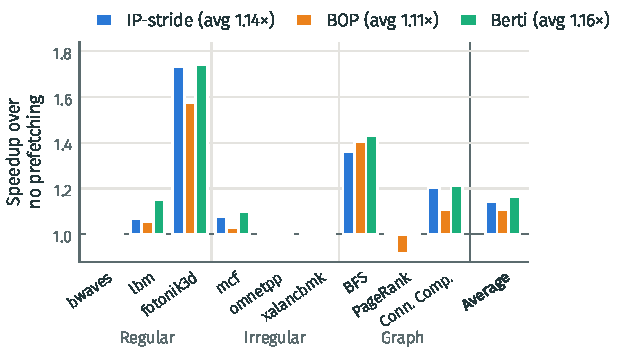
\includegraphics[width=\linewidth,height=0.56\textheight,keepaspectratio]{figs/speedup.pdf}
\end{frame}

% ---------------------------------------------------------------------------
\begin{frame}{Baselines: Accuracy}
  \centering
  \msg{\textbf{Berti stays accurate by staying silent;}\\
       BOP's guesses collapse on irregular and graph code}\\[0.3cm]
  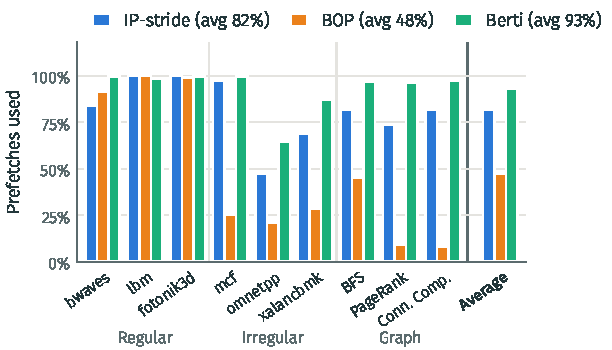
\includegraphics[width=\linewidth,height=0.56\textheight,keepaspectratio]{figs/accuracy.pdf}\\[0.1cm]
  {\scriptsize\color{black!55}Prefetches used = of all lines prefetched, the share the program actually used.}
\end{frame}

% ---------------------------------------------------------------------------
\begin{frame}{Q1: How Big Is the Gap?}
  \centering
  \msg{On irregular and graph code, \textbf{68--99\%} of Berti's misses\\
       happen while Berti is silent}\\[0.3cm]
  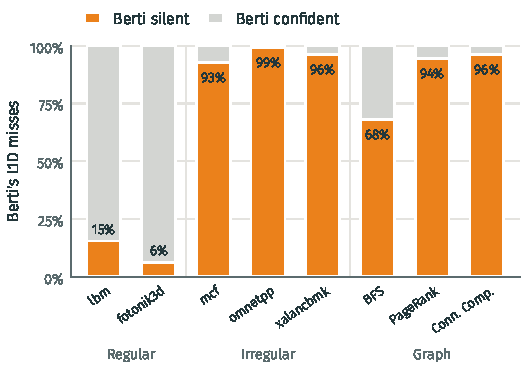
\includegraphics[width=\linewidth,height=0.56\textheight,keepaspectratio]{figs/gap.pdf}
\end{frame}

% ---------------------------------------------------------------------------
\begin{frame}{Q2 + Q3: Can a Global Offset Fill It?}
  \centering
  \msg{\textbf{Mostly no:} it catches $\le$30\% of silent misses,\\
       and $\le$37\% of its guesses are right}\\[0.3cm]
  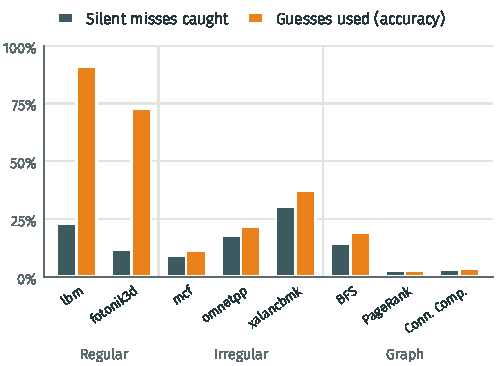
\includegraphics[width=\linewidth,height=0.56\textheight,keepaspectratio]{figs/fallback.pdf}\\[0.1cm]
  {\small Regular code: accurate guesses, but little left to catch}
\end{frame}

% ---------------------------------------------------------------------------
\begin{frame}{Who Causes the Gap?}
  \centering
  \msg{\textbf{A few hot instructions, not cold ones}}\\[0.3cm]
  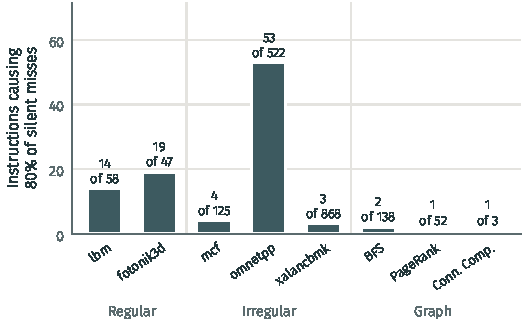
\includegraphics[width=\linewidth,height=0.56\textheight,keepaspectratio]{figs/concentration.pdf}\\[0.15cm]
  {\small Instructions with $<$1{,}000 loads cause $\le$0.2\% of silent misses\\
   on irregular and graph code}
\end{frame}

% ---------------------------------------------------------------------------
\begin{frame}{Key Takeaways}
  \centering
  \begin{tikzpicture}[
      tnum/.style={anchor=east, font=\LARGE\bfseries},
      tcap/.style={anchor=west, font=\normalsize, text=mDarkTeal},
      tlink/.style={anchor=west, font=\small\itshape, text=black!50}]
    % one subject throughout: Berti's silent misses
    \node[tnum, text=cBerti]      at (0, 0)    {93\%};
    \node[tcap] at (0.3, 0)       {of Berti's prefetches are right};
    \node[tlink] at (0.3,-0.62)   {\(\downarrow\) because it stays silent when unsure};

    \node[tnum, text=mLightBrown] at (0,-1.3)  {68--99\%};
    \node[tcap] at (0.3,-1.3)     {of its misses happen while it is silent};
    \node[tlink] at (0.3,-1.92)   {\(\downarrow\) a global offset fixes only};

    \node[tnum, text=mDarkTeal]   at (0,-2.6)  {\(\le\)30\%};
    \node[tcap] at (0.3,-2.6)     {of these silent misses};
    \node[tlink] at (0.3,-3.22)   {\(\downarrow\) but};

    \node[tnum, text=mDarkTeal]   at (0,-3.9)  {1--4};
    \node[tcap] at (0.3,-3.9)     {instructions cause 80\% of them};
  \end{tikzpicture}\\[0.5cm]
  \msg{\(\Rightarrow\) \textbf{Fix silent misses per instruction, not globally}}\\[0.2cm]
%   {\scriptsize\color{black!55}Irregular and graph code; 1--4 instructions on 5 of 8 traces.}
\end{frame}

% ---------------------------------------------------------------------------
\begin{frame}{Answer: It Depends on the Instruction}
  \centering
  {\large xalancbmk: the 4 loads with the most silent misses}\\[0.45cm]
  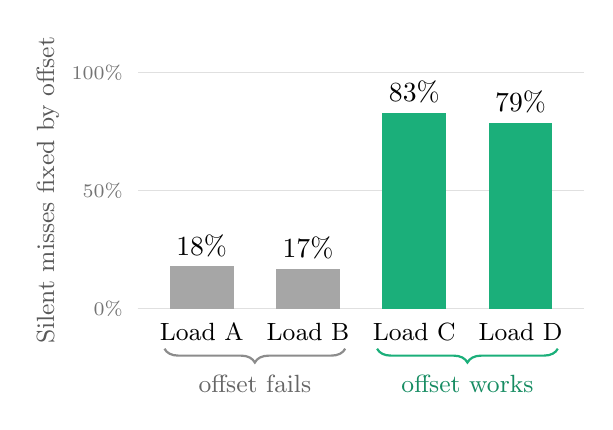
\begin{tikzpicture}[x=1.35cm, y=3.0cm,
      val/.style={font=\normalsize, anchor=south},
      brace/.style={decorate, decoration={brace, amplitude=5pt, mirror}, thick}]
    % axis
    \draw[black!40] (0.4,0) -- (4.6,0);
    \foreach \y/\t in {0/0\%, 0.5/50\%, 1/100\%} {
      \draw[black!12] (0.4,\y) -- (4.6,\y);
      \node[font=\scriptsize, text=black!55, anchor=east] at (0.35,\y) {\t};
    }
    \node[font=\small, text=black!65, rotate=90, anchor=south] at (-0.25,0.5)
      {Silent misses fixed by offset};
    % bars
    \foreach \i/\v/\c/\t/\n in {1/0.178/black!35/18/A, 2/0.167/black!35/17/B,
                                 3/0.827/cBerti/83/C, 4/0.786/cBerti/79/D} {
      \fill[\c] (\i-0.3,0) rectangle (\i+0.3,\v);
      \node[val] at (\i,\v) {\t\%};
      \node[font=\small, anchor=north] at (\i,-0.02) {Load \n};
    }
    % groups
    \draw[brace, black!45] (0.65,-0.17) -- (2.35,-0.17)
      node[midway, below=6pt, font=\small, text=black!60] {offset fails};
    \draw[brace, cBerti]   (2.65,-0.17) -- (4.35,-0.17)
      node[midway, below=6pt, font=\small, text=cBerti!80!black] {offset works};
  \end{tikzpicture}\\[0.5cm]
  \msg{\textbf{Same program, same offset}\\turn it on only for loads where it works}
\end{frame}

% ---------------------------------------------------------------------------
\begin{frame}[c]{Plan for Checkpoint 2}
  \begin{enumerate}[leftmargin=*, label={\huge\color{mLightBrown}\arabic*}, itemsep=22pt]
    \item {\Large \textbf{Measure:} for each load, how often\\the offset's guess is right}
    \item {\Large \textbf{Build LoGO:} a small table (8 loads, $\approx$30 bytes)\\
          that turns the offset on only where it is right}
    \item {\Large \textbf{Compare} LoGO with Berti and BOP:\\speed and accuracy}
  \end{enumerate}
\end{frame}

\begin{frame}[c]
    \centering
    {\Huge \textbf{Thank You!}}\\[1cm]
\end{frame}

\end{document}